\begin{figure}[t]
\centering

% ---------------- Latency ----------------
\begin{subfigure}{0.49\linewidth}
\centering
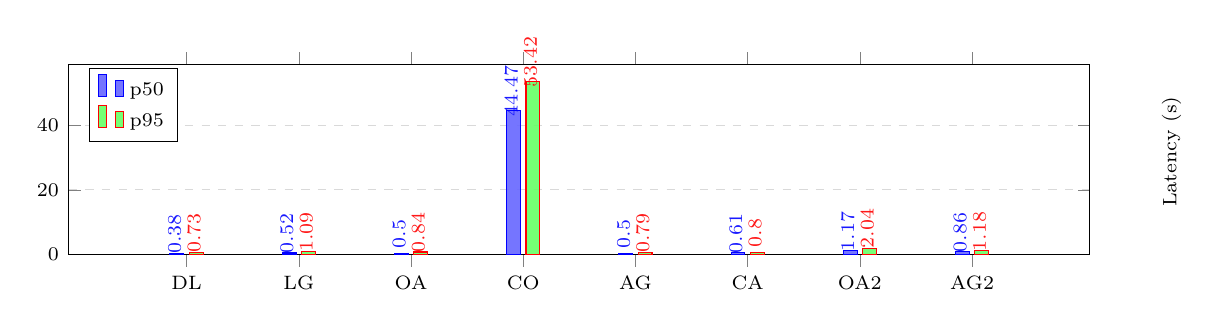
\begin{tikzpicture}
\begin{axis}[
    width=1.2\linewidth,
    height=4cm,
    ymin=0,
    symbolic x coords={DL,LG,OA,CO,AG,CA,OA2,AG2},
    xtick=data,
    ylabel={Latency (s)},
    ylabel style={at={(axis description cs:1.08,0.2)}, anchor=west},
    legend style={at={(0.02,0.98)}, anchor=north west, font=\scriptsize},
    tick label style={font=\scriptsize},
    ylabel style={font=\scriptsize},
    xlabel style={font=\scriptsize},
    ybar,
    bar width=5pt,
    enlarge x limits=0.15,
    ymajorgrids=true,
    grid style={dashed,gray!30},
    nodes near coords,
    nodes near coords style={
        font=\scriptsize,
        yshift=7pt,
        xshift=5pt,
        anchor=south,
        rotate=90
    },
    every axis plot/.append style={fill opacity=0.9}
]
\addplot+[fill=blue!60] coordinates {(DL,0.379) (LG,0.524) (OA,0.495) (CO,44.473) (AG,0.496) (CA,0.611) (OA2,1.170) (AG2,0.860)};
\addplot+[fill=green!60] coordinates {(DL,0.730) (LG,1.093) (OA,0.840) (CO,53.420) (AG,0.787) (CA,0.801) (OA2,2.036) (AG2,1.183)};
\legend{p50, p95}
\end{axis}
\end{tikzpicture}
\caption{Latency}
\end{subfigure}
\hfill

% ---------------- Throughput ----------------
\begin{subfigure}{0.49\linewidth}
\centering
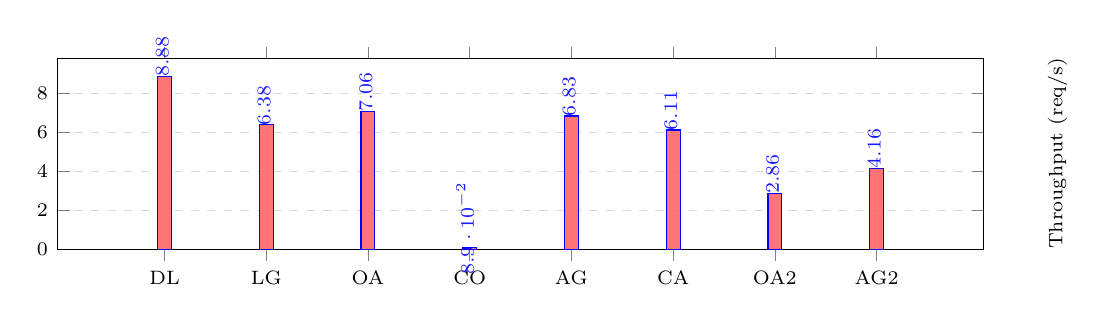
\begin{tikzpicture}
\begin{axis}[
    width=1.1\linewidth,
    height=4cm,
    ymin=0,
    symbolic x coords={DL,LG,OA,CO,AG,CA,OA2,AG2},
    xtick=data,
    ylabel={Throughput (req/s)},
    ylabel style={at={(axis description cs:1.08,-0.05)}, anchor=west},
    tick label style={font=\scriptsize},
    ylabel style={font=\scriptsize},
    xlabel style={font=\scriptsize},
    ybar,
    bar width=5pt,
    enlarge x limits=0.15,
    ymajorgrids=true,
    grid style={dashed,gray!30},
    nodes near coords,
    nodes near coords style={
        font=\scriptsize,
        yshift=7pt,
        xshift=5pt,
        anchor=south,
        rotate=90
    },
    every axis plot/.append style={fill opacity=0.9}
]
\addplot+[fill=red!60] coordinates {(DL,8.875) (LG,6.377) (OA,7.062) (CO,0.089) (AG,6.827) (CA,6.113) (OA2,2.860) (AG2,4.158)};
\end{axis}
\end{tikzpicture}
\caption{Throughput}
\end{subfigure}

\vspace{0.6em}

% ---------------- Mean Output ----------------
\begin{subfigure}{0.49\linewidth}
\centering
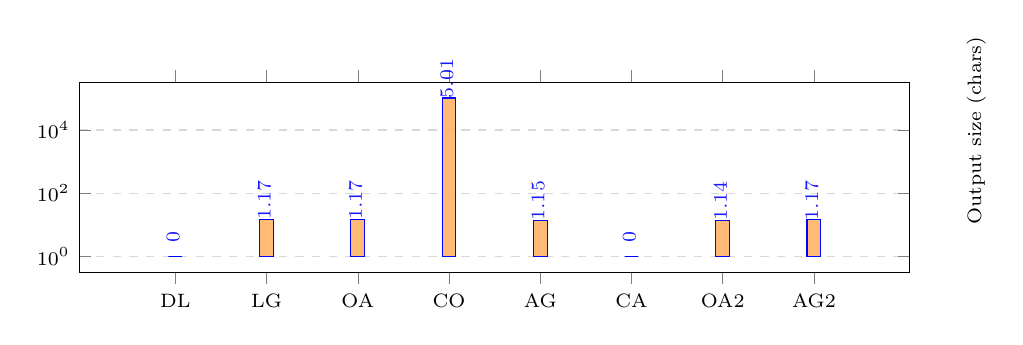
\begin{tikzpicture}
\begin{axis}[
    width=1.0\linewidth,
    height=4cm,
    ymode=log,
    log basis y=10,
    symbolic x coords={DL,LG,OA,CO,AG,CA,OA2,AG2},
    xtick=data,
    ylabel={Output size (chars)},
    ylabel style={at={(axis description cs:1.08,0.2)}, anchor=west},
    tick label style={font=\scriptsize},
    ylabel style={font=\scriptsize},
    xlabel style={font=\scriptsize},
    ybar,
    bar width=5pt,
    enlarge x limits=0.15,
    ymajorgrids=true,
    grid style={dashed,gray!30},
    nodes near coords,
    nodes near coords style={
        font=\scriptsize,
        yshift=7pt,
        xshift=5pt,
        anchor=south,
        rotate=90
    },
    every axis plot/.append style={fill opacity=0.9}
]
\addplot+[fill=orange!60] coordinates {(DL,1.000) (LG,14.900) (OA,14.900) (CO,102601.360) (AG,14.220) (CA,1.000) (OA2,13.880) (AG2,14.800)};
\end{axis}
\end{tikzpicture}
\caption{Mean output}
\end{subfigure}
\hfill

% ---------------- Output Summary ----------------
\begin{subfigure}{0.49\linewidth}
\centering
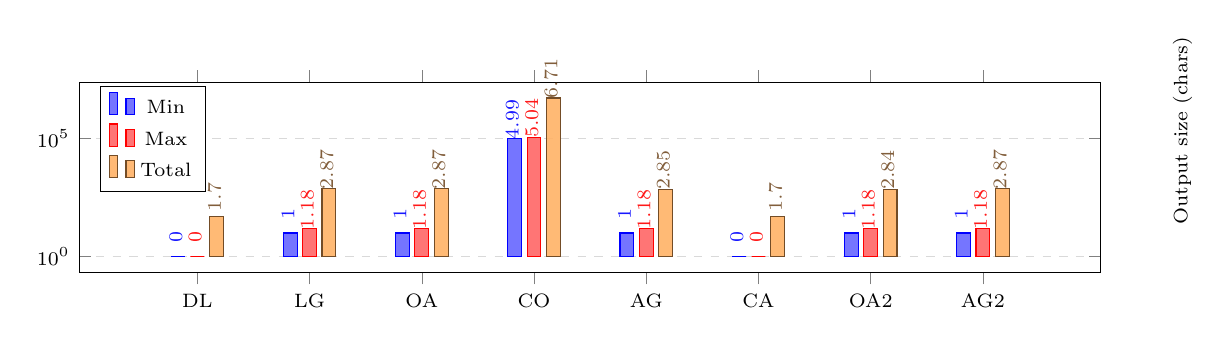
\begin{tikzpicture}
\begin{axis}[
    width=1.2\linewidth,
    height=4cm,
    ymode=log,
    log basis y=10,
    symbolic x coords={DL,LG,OA,CO,AG,CA,OA2,AG2},
    xtick=data,
    ylabel={Output size (chars)},
    ylabel style={at={(axis description cs:1.08,0.2)}, anchor=west},
    legend style={at={(0.02,0.98)}, anchor=north west, font=\scriptsize},
    tick label style={font=\scriptsize},
    ylabel style={font=\scriptsize},
    xlabel style={font=\scriptsize},
    ybar,
    bar width=5pt,
    enlarge x limits=0.15,
    ymajorgrids=true,
    grid style={dashed,gray!30},
    nodes near coords,
    nodes near coords style={
        font=\scriptsize,
        yshift=7pt,
        xshift=5pt,
        anchor=south,
        rotate=90
    },
    every axis plot/.append style={fill opacity=0.9}
]
\addplot+[fill=blue!60] coordinates {(DL,1.000) (LG,10.000) (OA,10.000) (CO,97448.000) (AG,10.000) (CA,1.000) (OA2,10.000) (AG2,10.000)};
\addplot+[fill=red!60] coordinates {(DL,1.000) (LG,15.000) (OA,15.000) (CO,110886.000) (AG,15.000) (CA,1.000) (OA2,15.000) (AG2,15.000)};
\addplot+[fill=orange!60] coordinates {(DL,50.000) (LG,745.000) (OA,745.000) (CO,5130068.000) (AG,711.000) (CA,50.000) (OA2,694.000) (AG2,740.000)};
\legend{Min, Max, Total}
\end{axis}
\end{tikzpicture}
\caption{Output summary}
\end{subfigure}

\caption{Framework overhead results for 50 trials of the trivial task (``What is 2+2?''). 
\textbf{DL} = Direct LLM, \textbf{LG} = LangGraph, \textbf{OA} = OpenAgents, \textbf{CO} = Concordia, \textbf{AG} = AutoGen, \textbf{CA} = CrewAI, \textbf{OA2} = OpenAISDK, \textbf{AG2} = Agno.}
\label{fig:framework-overhead}
\end{figure}